\documentclass{astroedu-lab}

\begin{document}

\pagestyle{plain}

\begin{problem}{\huge Лабораторная работа 2.5.1\\\\Измерение коэффициента\\\\поверхностного натяжения жидкости\\\\Выполнил Жданов Елисей Б01-205}

\section{Цель работы:}

1) Измерение температурной зависимости  коэффициента поверхностного натяжения дистиллированной воды с использованием известного коэффициента поверхностного натяжения спирта.

2) Определение полной поверхностной энергии  и теплоты, необходимой для изотермического образования единицы  поверхности жидкости при различной температуре. 

\section{Оборудование:}

Прибор  Ребиндера  с термостатом и микроманометром

Исследуемые жидкости

Стаканы

\section{Теоретическая справка}

Для сферического пузырька с воздухом  внутри жидкости избыточное давление задаётся формулой Лапласа:

\begin{equation}
	\Delta P = P_{\text {внут}}-P_{\text {снар}}=\frac{2 \sigma}{r}	
\end{equation}

где $\sigma$ – коэффициент поверхностного натяжения, r – радиус кривизны поверхности раздела двух фаз.

По полученной зависимости $\sigma(T)$ можно определить величины теплоты образования единицы поверхности жидкости:
\[
q = -T \frac{d\sigma}{d T}
\]

а также поверхностной энергии U единицы площади F:

\begin{equation}
	\frac{U}{F} = \left( \sigma - T \frac{d \sigma}{d T} \right)
\end{equation}
 
\section{Экспериментальная установка}

\begin{figure}[!h]
	\centering
	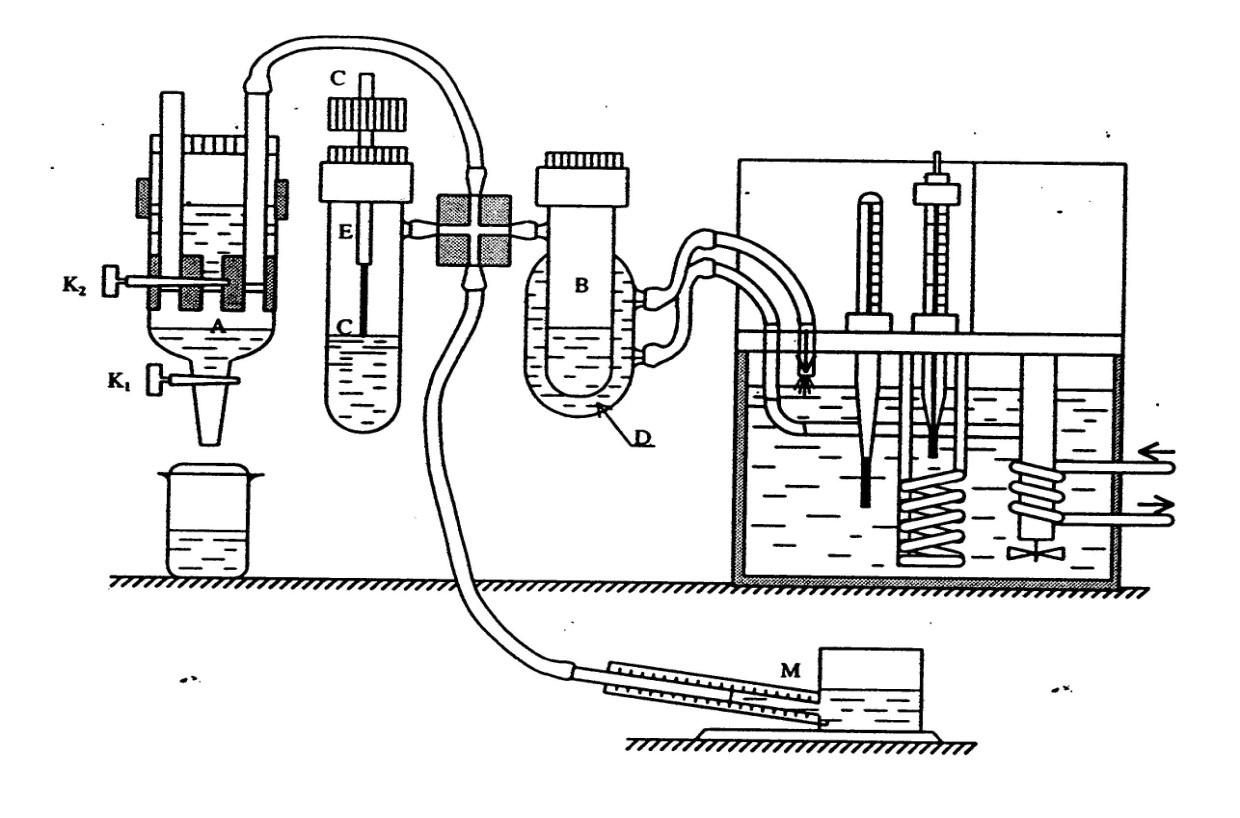
\includegraphics[width=0.9\textwidth]{pic1.png}
	\label{fig:boiler}
\end{figure}

Дистиллированная вода наливается в сосуд В. Этиловый спирт наливается в сосуд Е.

При измерениях  колбы герметично закрываются  пробками. Через одну из двух пробок  проходит полая металлическая игла С. Этой пробкой закрывается сосуд, в котором  проводятся измерения. Верхний конец иглы открыт в атмосферу, а нижний погружен в жидкость.

Другой сосуд герметично закрывается второй пробкой. При создании достаточного  разряжения воздуха в колбе с иглой пузырьки воздуха начинают пробулькивать через жидкость. Поверхностное натяжение можно определить по величине разряжения $\Delta P$, необходимого для прохождения пузырьков.

\section{Измерения, Обработка}

\subsection{Измерения диаметра в спирте}

В начале работы необходимо убедиться в точной калибровке манометра, определить нуль его шкалы и в дальнейшем производить замеры, определяя одинаковым методом показания столбика спирта в нем.

Установим иглу в пробирку со спиртом и соприкоснем её с поверхностью этанола. Откроем кран К1.

5 измерений манометра дали одинаковые результаты

\[
	h _\text{ман, этанол} = (43 \pm 1) \text{ мм}
\]

Используем формулу для пересчета высоты столба спирта в манометре в разность давлений

\begin{equation}
	\frac{2 \sigma}{r} = \Delta P = g k h_\text{ман}
\end{equation}

k = 0.2

Согласно ей, принимая комнатную температуру за 22.3 $^\circ$ С, а следовательно, $\sigma_\text{этанол} = \frac{(30.0 - 22.3) \cdot 22.78 + (22.3 - 20.0) \cdot 21.90}{10} = 22.58 \frac{\text{мН}}{\text{К}}$ (линейная интерполяция), получим

\begin{equation}
	2r = d = \frac{4 \sigma}{g k h_\text{ман}} = (1.07 \pm 0.02) \text{ мм}
\end{equation}

Погрешность определяется только величиной $h_\text{ман}$

\begin{equation}
	\varepsilon_{r} = \varepsilon_{h_\text{ман}}
\end{equation}

\subsection{Измерения диаметра микроскопом}

Также диаметр иглы можно измерить визуально с помощью микроскопа.

Результат

\[
d = (1.15 \pm 0.05) \text{ мм}
\]

Полученные разными методами значения d совпадают в пределах погрешности. К тому же справедливо отметить, что для нахождения величины $\sigma$ следует использовать "гидростатический" радиус иглы, а не оптический. Поэтому в дальнейшем первое значение будет использоваться в расчетах.

\subsection{Измерения глубины погружения в воде}

Просушим и продуем иглу от спирта и установим в пробирку с водой.

Приведем замеры нужных величин для иглы, соприкасающейся с поверхностью воды

Относительная высота иглы $h1 = (53 \pm 1) \text{ мм}$

Показания манометра для максимального давления $h1 _\text{ман} = (116 \pm 1) \text{ мм}$

Далее погрузим иглу и найдём теже величины:

Относительная высота иглы $h2_\text{max} = (40 \pm 1) \text{ мм}$

Показания манометра для максимального давления $P2_\text{max} = (188 \pm 1) \text{ мм}$

Теперь определим глубину погружения иглы в воду для корректировки абсолютных значений давления

Линейно: $\Delta h = h_1 - h_2 = (13.0 \pm 1.4) \text{ мм}$

Гидростатически: $\Delta h = \frac{k (h2 _\text{ман} - h1 _\text{ман})}{\rho} = (14.4 \pm 0.3)$

Погрешность определяется таким образом

\begin{equation}
	\sigma_{\Delta h} = \sqrt{\sigma_{h1}^2 + \sigma_{h2}^2}
\end{equation}

и

\begin{equation}
	\sigma_{\Delta h} = \sqrt{\sigma_{h1}^2 + \sigma_{h2}^2} \cdot  \frac{k}{\rho}
\end{equation}

Как результат, разница в 10$\%$ может быть сочтена как погрешность обеих методик.

\subsection{Измерения $\sigma(T)$ в воде}

Теперь будем снимать зависимость $\sigma(T)$, убедившись, что прибор откалиброван после прошедших манипуляций.

Для расчета $\sigma$ выразим её через $h_\text{ман}$

\begin{equation}
	\sigma_{H_2 O} = \frac{g k (h_\text{ман} - h_{H_2 O}) d}{4}
\end{equation}

Высота $h_{H_2 O}$ есть величина смещения показаний манометра из-за погружения в воду иглы. Её следует пересчитать через найденную линейную $\Delta h$.

То бишь

\begin{equation}
	h_{H_2 O} = \frac{\Delta h \rho}{k} = (65 \pm 7) \text{ мм}
\end{equation}

Тогда занесем все полученные и пересчитанные данные в таблицу

\begin{center}
\begin{tabular}{|c|c|c|c|}
\hline 
\multicolumn{2}{|c|}{$h_\text{ман}$, мм} & $\sigma, \frac{\text{мН}}{\text{К}}$ & T, $^\circ$C \\
\hline
188.0 & 188.0 & $(64.5 \pm 3.9)$ & 22\\
187.0 & 187.0 & $(64.0 \pm 3.9)$ & 30\\
185.5 & 186.0 & $(63.3 \pm 3.9)$ & 35\\
184.0 & 184.5 & $(62.5 \pm 3.9)$ & 40\\
182.5 & 183.0 & $(61.7 \pm 3.9)$ & 45\\
181.0 & 181.0 & $(60.8 \pm 3.8)$ & 50\\
179.0 & 179.5 & $(59.9 \pm 3.8)$ & 55\\
177.5 & 177.5 & $(59.0 \pm 3.8)$ & 60\\
\hline
\end{tabular}
\end{center}

Построим график зависимости $\sigma(T)$

Первую точку(комнатная температура) выбросим, она сильно отклоняется от остальных.

\begin{center}
	\text{\Large $\sigma(T)$}
\end{center}

\begin{figure}[!h]
	\centering
	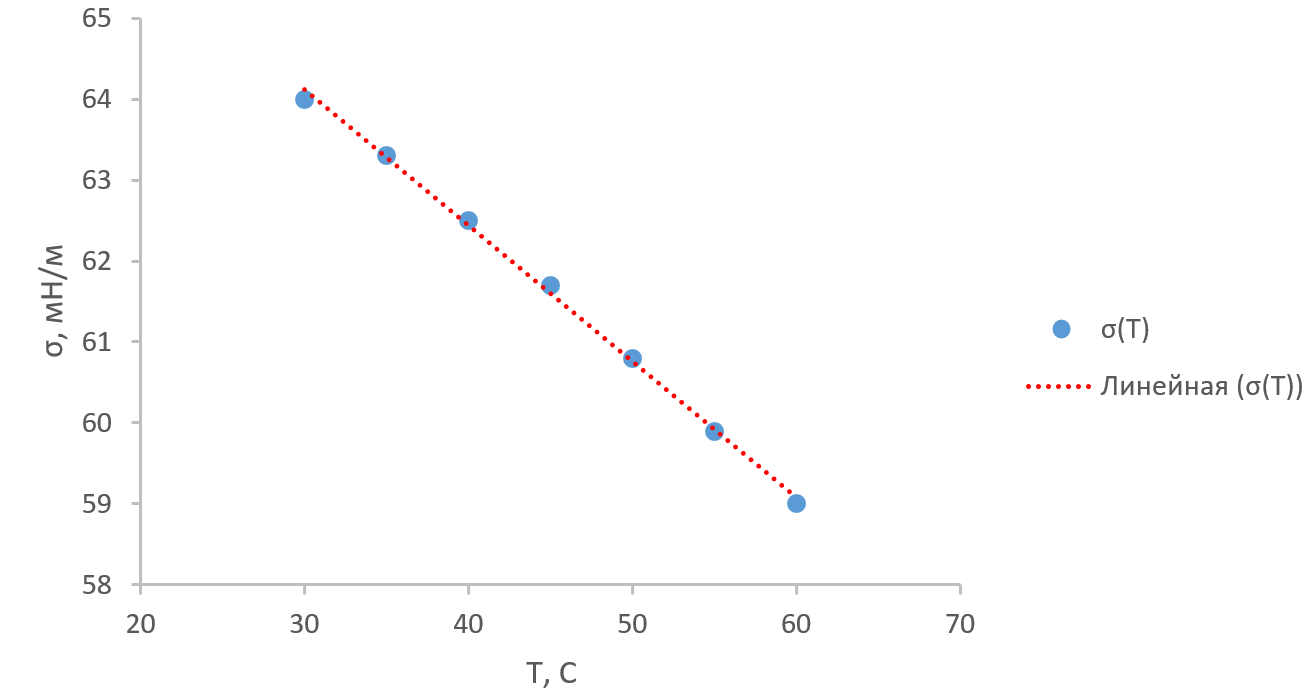
\includegraphics[width=1\textwidth]{2023-02-23_21-33-13.png}
	\label{fig:boiler}
\end{figure}

\newpage

\begin{figure}[!h]
	\centering
	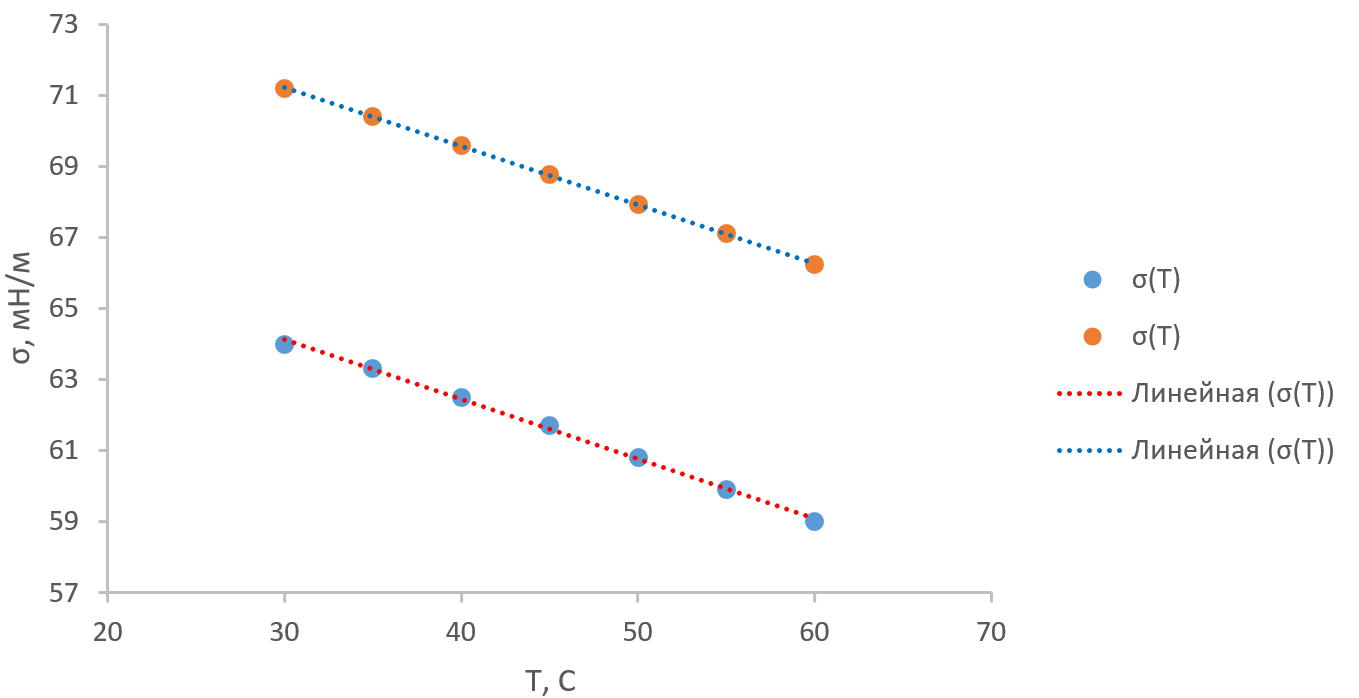
\includegraphics[width=1\textwidth]{2023-02-23_22-55-47.png}
	\label{fig:boiler}
\end{figure}

Найдем угловые коэффициенты прямых для каждой установки по МНК.

\[
	a = \frac{<x_i y_i> - < x > < y_i >}{< x_i^2> - < x_i >^2}
\]

\[
	b = < \nu_i > - a < N_i >
\]

Также рассчитаем их погрешности

\begin{equation}
	S_a^2 = \frac{< x_i^2>}{< x_i^2 > - < x_i >^2} \cdot \frac{<  b_i - b > ^2}{n - 2}
\end{equation}

Итоговая формула зависимости

\[
	\sigma = (69.2 \pm 3.9) - (0.1679 \pm 0.0032)T
\]

\begin{center}
	$\sigma \left[ \frac{\text{мН}}{\text{К}} \right]$, а $T \left[ ^\circ C \right]$
\end{center}

При этом погрешность при свободном члене пересчитана с учетом погрешностей $\sigma_i$

Соответствующий температурный коэффициент

\begin{equation}
	\frac{d \sigma}{d T} = -0.1679 \pm 0.0032 
\end{equation}

Построим требуемые графики q и $\frac{U}{F}$

\newpage

\begin{center}
	\Large $q(T)$
\end{center}

\begin{figure}[!h]
	\centering
	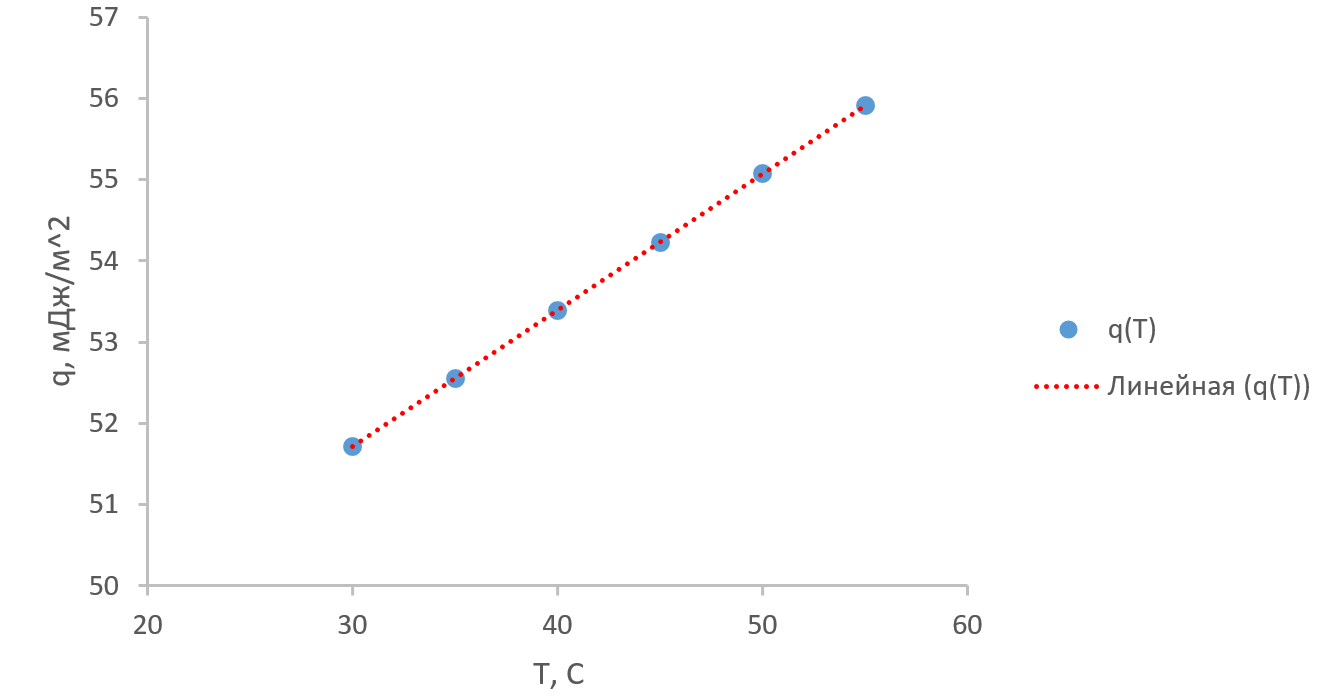
\includegraphics[width=1\textwidth]{2023-02-23_22-23-59.png}
	\label{fig:boiler}
\end{figure}

\begin{center}
	\Large $\frac{U}{F}(T)$
\end{center}

\begin{figure}[!h]
	\centering
	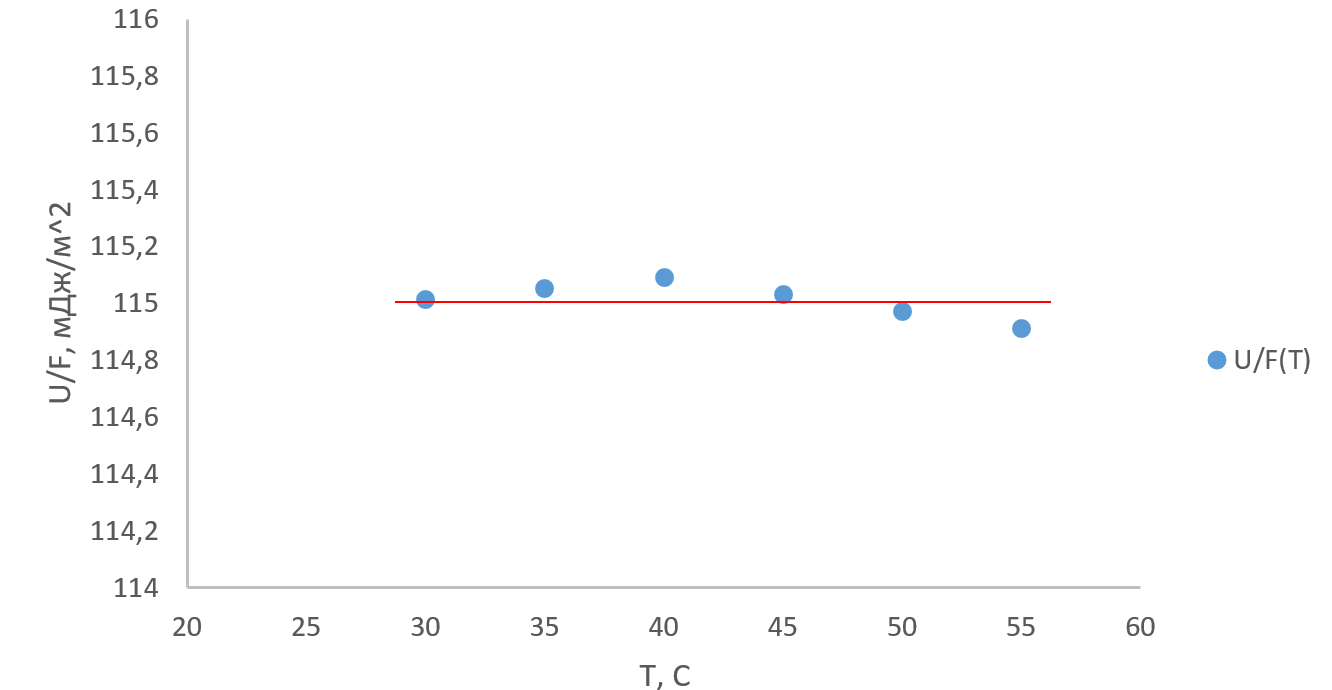
\includegraphics[width=1\textwidth]{2023-02-23_22-26-14.png}
	\label{fig:boiler}
\end{figure}

\section{Вывод}

В работе была исследована зависимость коэффициента поверхностного натяжения дистиллированной воды с использованием известного коэффициента поверхностного натяжения спирта.

В результате была получена линейная зависимость, отличающаяся от табличных значений не более чем на $10\%$.

Зависимость $q(T)$ получилась линейной, $\frac{U}{F}(T)$ - константной. Все это согласуется с теоретическими сведениями.

Среднее значение составляет $\frac{U}{F} = (115 \pm 4) \frac{\text{мДж}}{\text{м}^2}$


\section{Ресурсы}

Расчет по МНК: метод-наименьших-квадратов.рф


\end{problem}
\end{document}